\chapter{Development of the System}
\textit{In  this  chapter  we  will address  the  topics  of  stress management system development.  Discusses the development of the application and all elements which We  have  been used to implement the system for stress management at the  workplace  in  particular  for people with mental deficiency.}
\vspace{5mm}

A stress management application named \textbf{Schneckenhaus} has been developed to achieve the aim and objective of the research which is to decrease the stress level and empower the users of this system. 

Schneckenhaus is the German name of snail shell. We used this \textbf{Schneckenhaus} as metaphor of our stress management system. Thinking slow and brain function problems concept as a human organ in a snail shell as a mental health symbol for struggling with memory and dementia as alzheimer or neurology challenges \citep{Zachos2018TraumaResearch}.

The feeling stressed most of the time in workplace which we have focused on in the initial phase of the thesis was a Chronic stress disorder. “Chronic stress is the reaction to emotional pressure that has been experiencing for an extended period of time when a person perceives that they have little or no control. It involves an endocrine response to the system which releases corticosteroids. While in a single short-term situation the immediate effects of stress hormones are beneficial, long-term stress exposure creates a high level of those hormones. This can lead to high blood pressure (and eventually heart disease), muscle tissue damage, growth inhibition, immune system suppression \citep{Carlson2013PhysiologyBehavio} and mental health damage." \citep{Wiki2019ChronicWikipedia}. An extensive literature review has been done in order to get ourselves aware of the problem in detail before we actually started developing the application.

But later after the discussion with supervisors, we have decided not to move forward with stress disorder detection because this problem should be diagnosed by special medical procedure instructed by doctors among the people in our target user group. Our main focus is to build user's friendly stress management application for that we can focus on any stress management which is more common among the people. Dr. Benjamin Tannert proposed an idea of technology for special needs people.Suggested me to make an application which will be functional and help special needs people in reality. In the next section of this chapter, we will talk about the platform of the application which is in our case is stress management application \acf{UX} design, then we will describe the \acf{UI} development of the android application integrated with Smart \acs{IoT}.
\section{System Design}
System design is the process of designing the elements of a system such as the architecture, modules and devices, the different interfaces of those components and the data flowing through that system. 

The aim of the system design process in our thesis is to provide sufficient detailed data and information about the system and its system elements to allow implementation consistent with the architectural entities as described in system architecture models and views.

Making system design more specific first we design \acf{UX} and the we develop \acf{UI}.
\subsection{\acf{UX}}
Designing user experience is a human-first process of product design. A cognitive scientist and co-founder of the Nielsen Norman Group Design Consultancy, Don Norman has been credited with coining the term "user experience" in the late 1990s. He defines it this way:

    \say{User experience encompasses all aspects of the end-user’s interaction with the company, its services, and its products.}
– Don Norman, Cognitive Scientist \& User Experience Architect \citep{Norman1988TheThings}

We use persona analysis result and paper prototype outcome to design \acf{UX}  for our stress management system \textbf{Schneckenhaus}. Considering \acf{UX} In the next section we will discuss about \acf{UI} development.

\subsection{\acf{UI}}
\begin{figure}[hbt!] 
  \centering
  \subbottom[App welcome Screen]{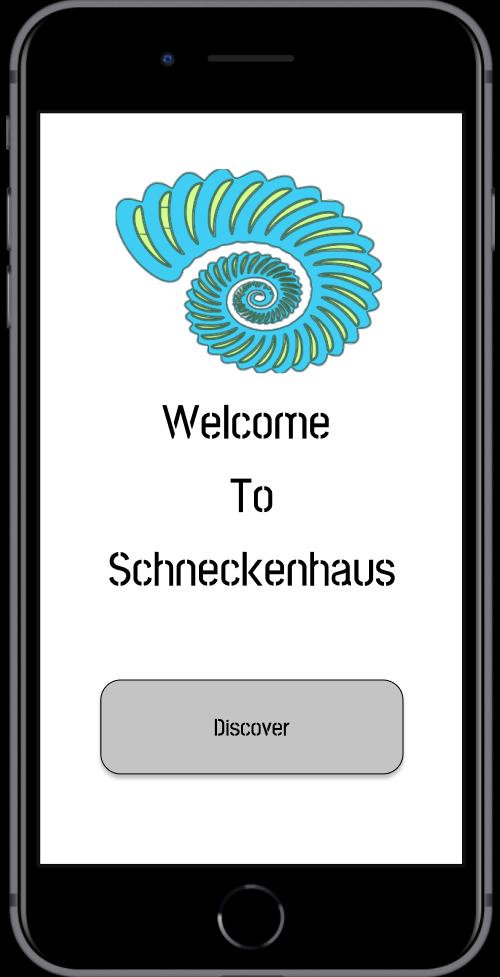
\includegraphics[width=0.45\textwidth]{chap4/image4/sc1.png}}\qquad
    \subbottom[main menu]{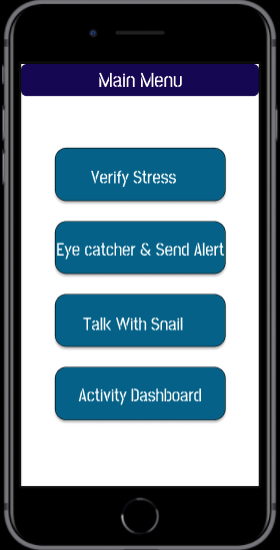
\includegraphics[width=0.45\textwidth]{chap4/image4/SC2.png}}
  \caption[\acf{UI} for Stress management System (1st and 2nd Screen)]{\acf{UI} for Stress management System (1st and 2nd Screen)\index{Hasnain}}
  \label{fig:S1}
\end{figure}

Schneckenhaus is an android application which is being developed using the latest coding language, standards, and practices of Android Programming. The programming language which  has been used to develop this app is Kotlin. 

According to Kotlin's official website "Kotlin is a cross-platform, statically typed, general-purpose programming language with type inference. Kotlin is designed to interoperate fully with Java, and the JVM (Java Virtual  Machine) version. 'In Google I / O 2017, Google officially supported Kotlin for mobile development in Android. And the company also encouraged Android Developers to start developing their apps in Kotlin. After the discussion with supervisors, it was decided that Schneckenhaus will be  developed in Kotlin, not in Java. 

In this section, we will talk about the implementation of each design of the application and also about  the part of the application which is same for all the design alternatives.  made a design alternative.  We didn't want to build a separate application for each condition Therefore, In figure:\ref{fig:S1}, (a) welcome screen and (b) all four \acs{UI} designs were incorporated into one single app through Main menu Screen As you see. This is the research project and the purpose of building this app was not to publish it on  Google Play Store or to use it for commercial purpose.  This app will be used in a research study which has four conditions, for each of the study's condition, we have (Activity).

In the next section I will discuss about four \acf{UI} menu development process and functionality.

\section{Verify Stress}
\begin{figure}[hbt!] 
  \centering
  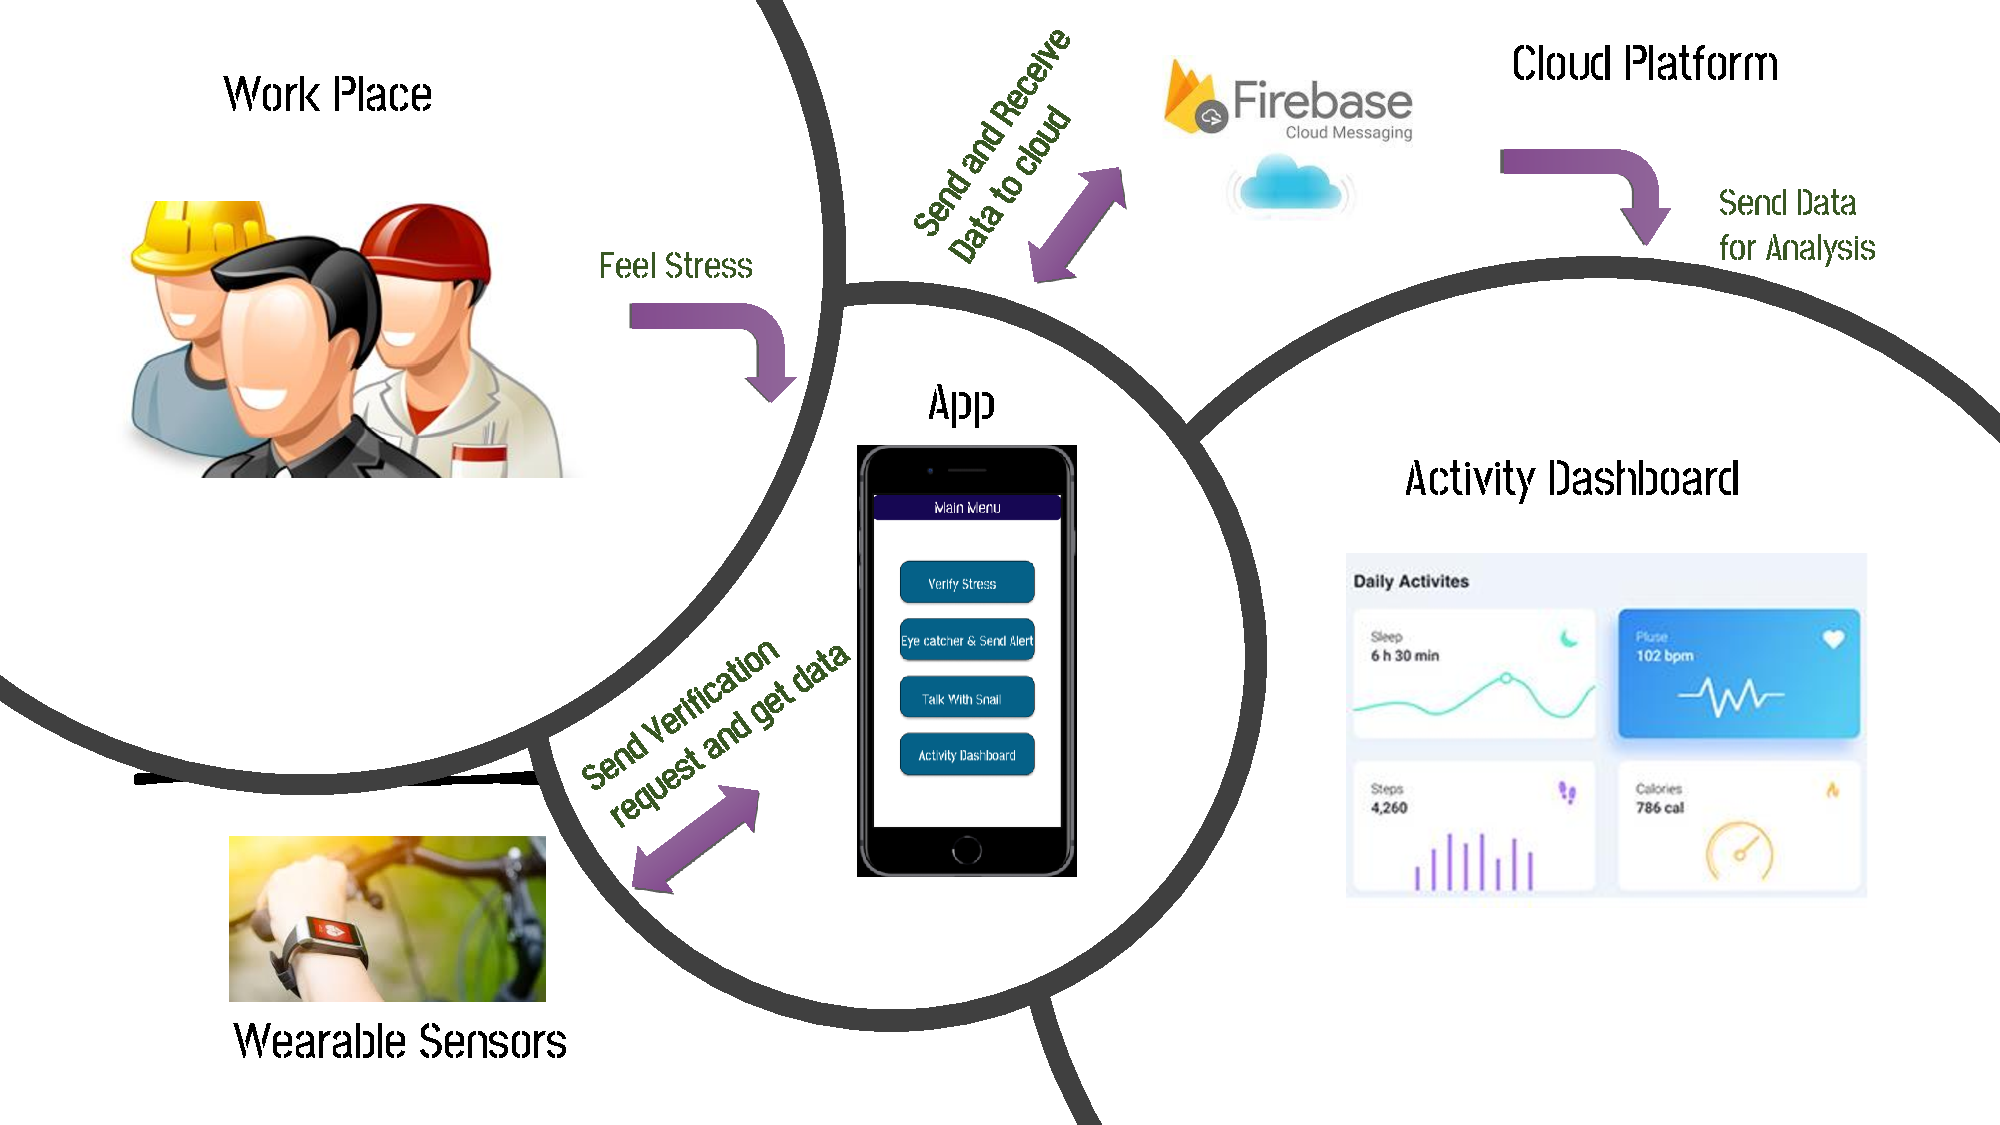
\includegraphics[width=1.0\linewidth]{chap4/image4/firbase.pdf}
  \caption[Verify Stress Process Diagram ]{Verify Stress Process Diagram\index{Hasnain}}
  \label{fig:Verify_Stress}
\end{figure}
In  this  research,  we  want  to  design  and  implement a system  to verify the psychophysiological signals monitoring stress during workplace and send data to cloud for analysis. 

In the work place when you feel the stress they can immediately go to the app then press verify stress option. Figure: \ref{fig:Verify_Stress} shows the whole presses diagram of Verify Stress Activity.App will give two different type health data from \acs{IoT} sensors.

\begin{itemize}
    \item 1. Heart rate sensor
    \item 2. \acf{SpO2} Sensor
\end{itemize}

In measuring health status, sensors and smart phones usually imply: collecting sensor data; providing user support through a display with the measured values; sharing information; ensuring low power devices, wear-ability, accuracy, durability and system reliability.

\subsection{Smart watch Heart rate sensor}
\begin{figure}[hbt!] 
  \centering
  \subbottom[Front view]{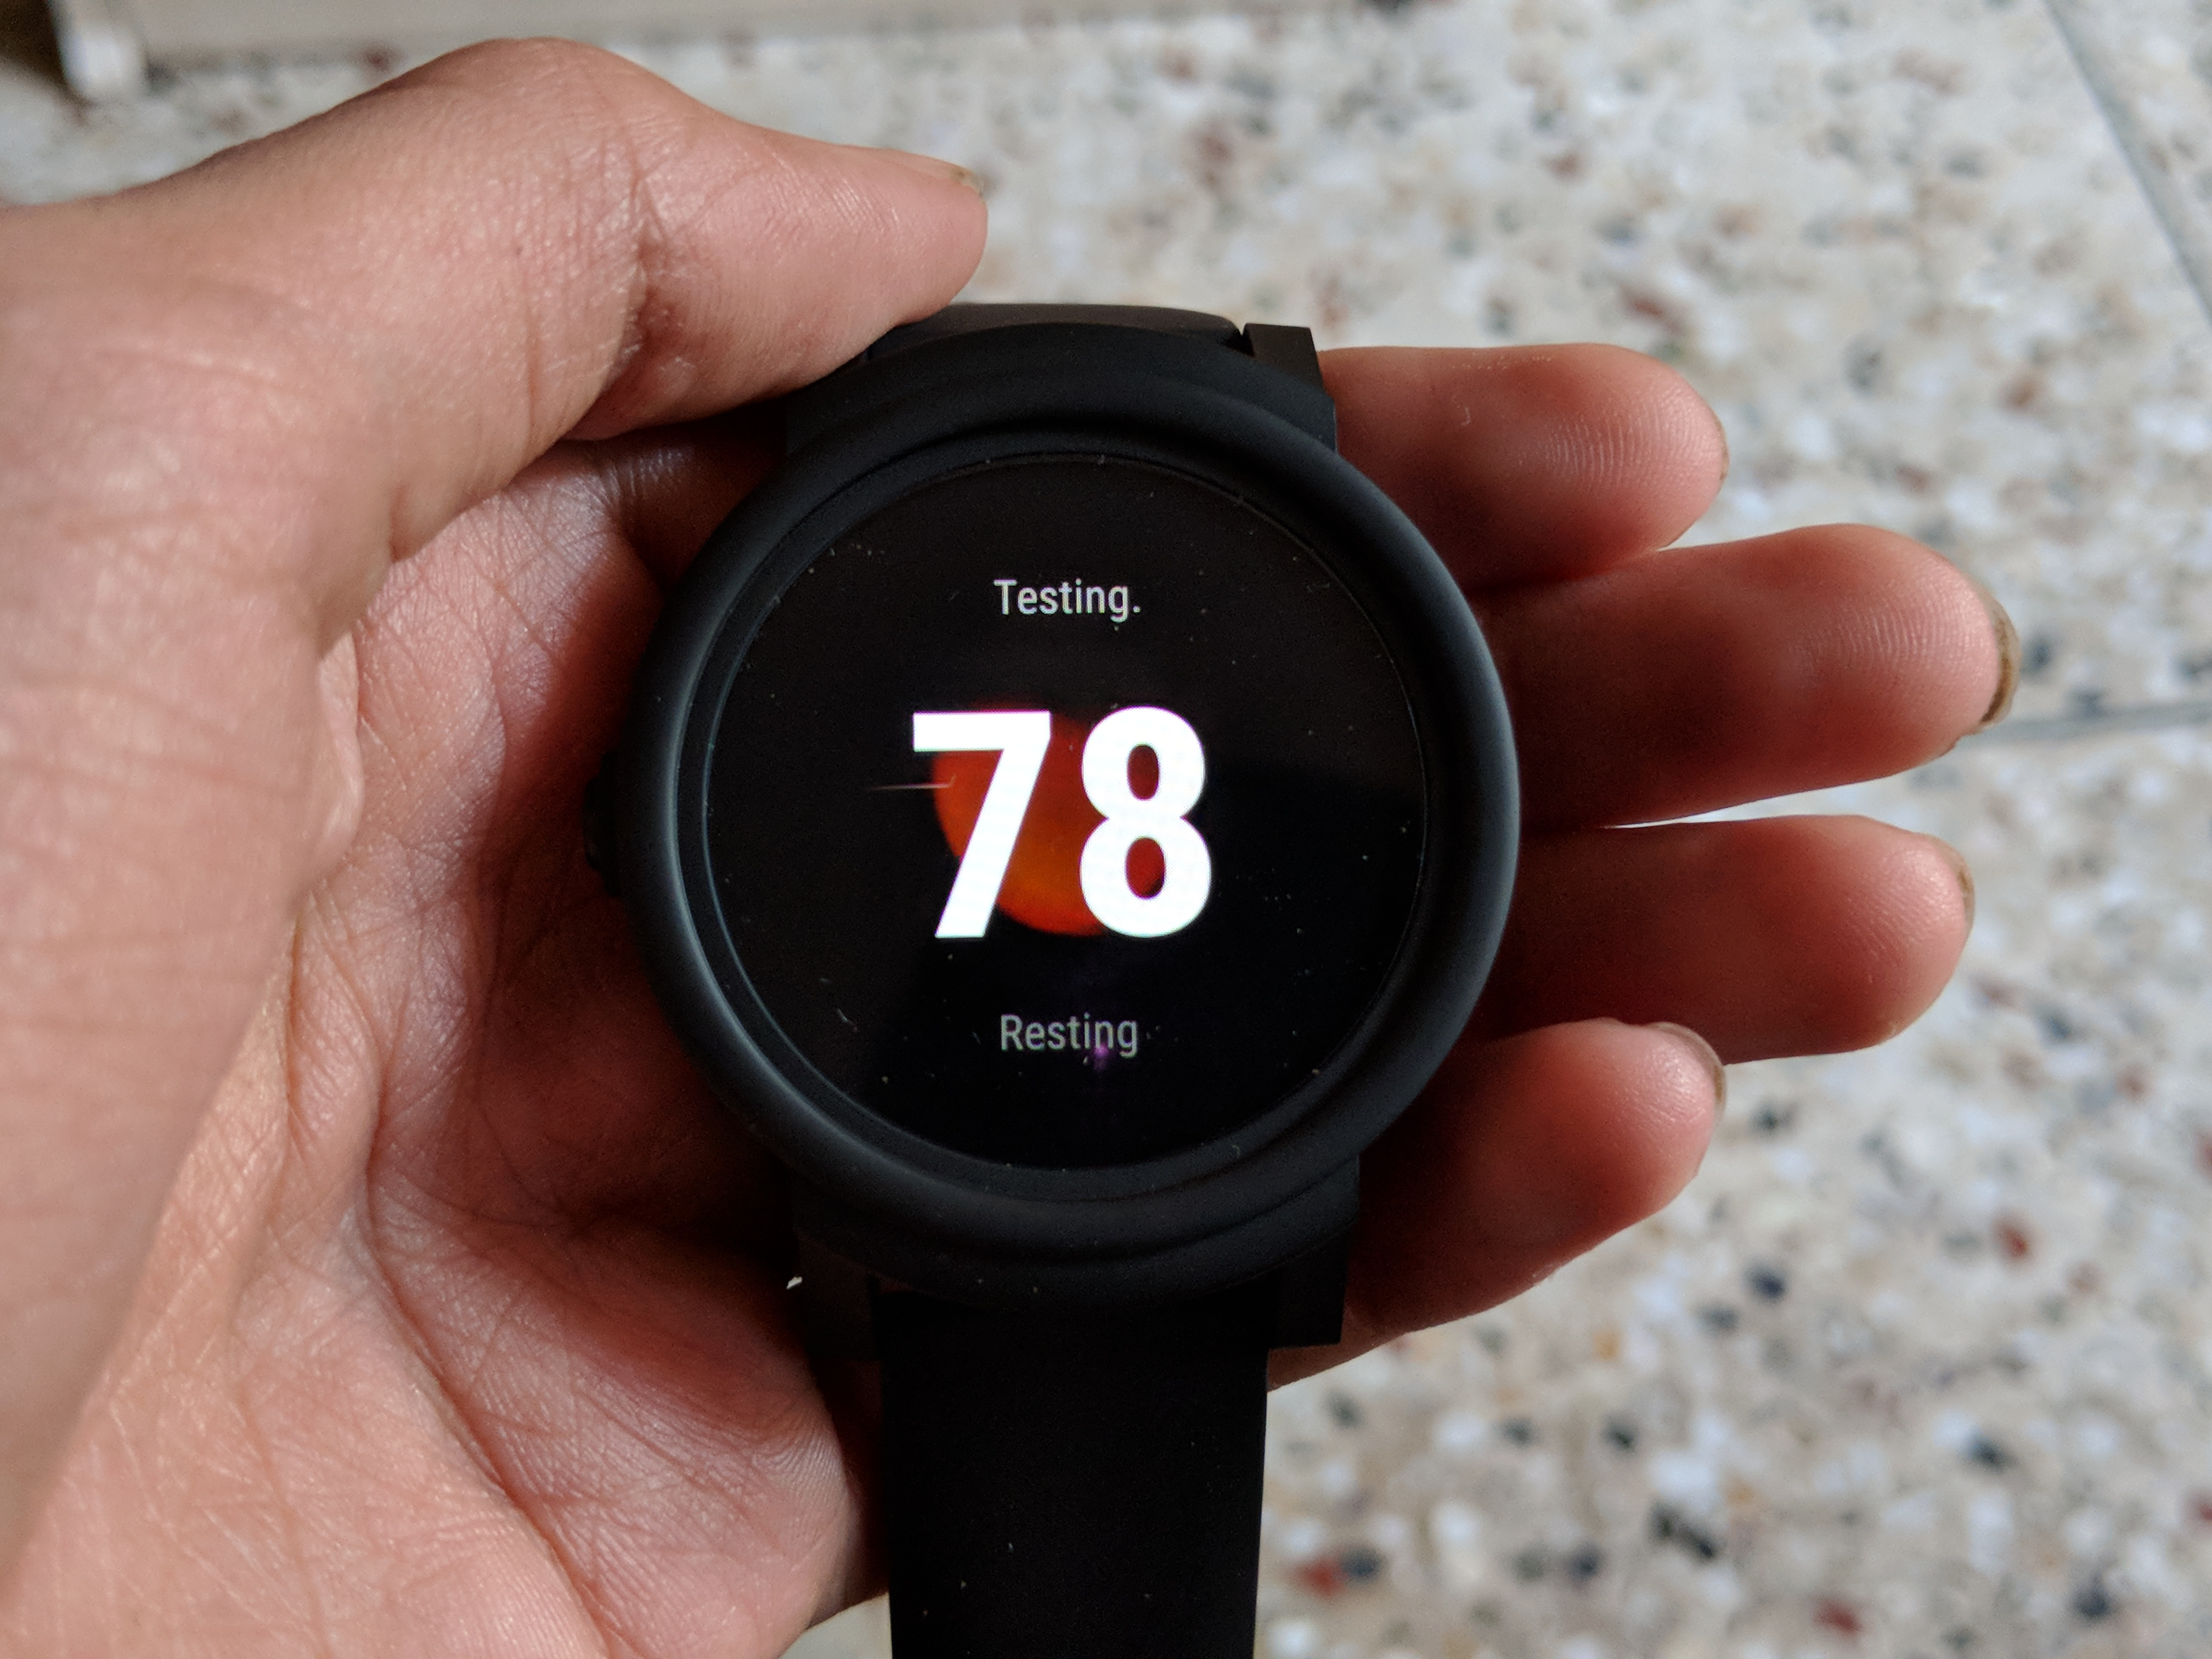
\includegraphics[width=0.45\textwidth]{chap4/image4/tikwatch.jpg}}\qquad
    \subbottom[Back side sensor view]{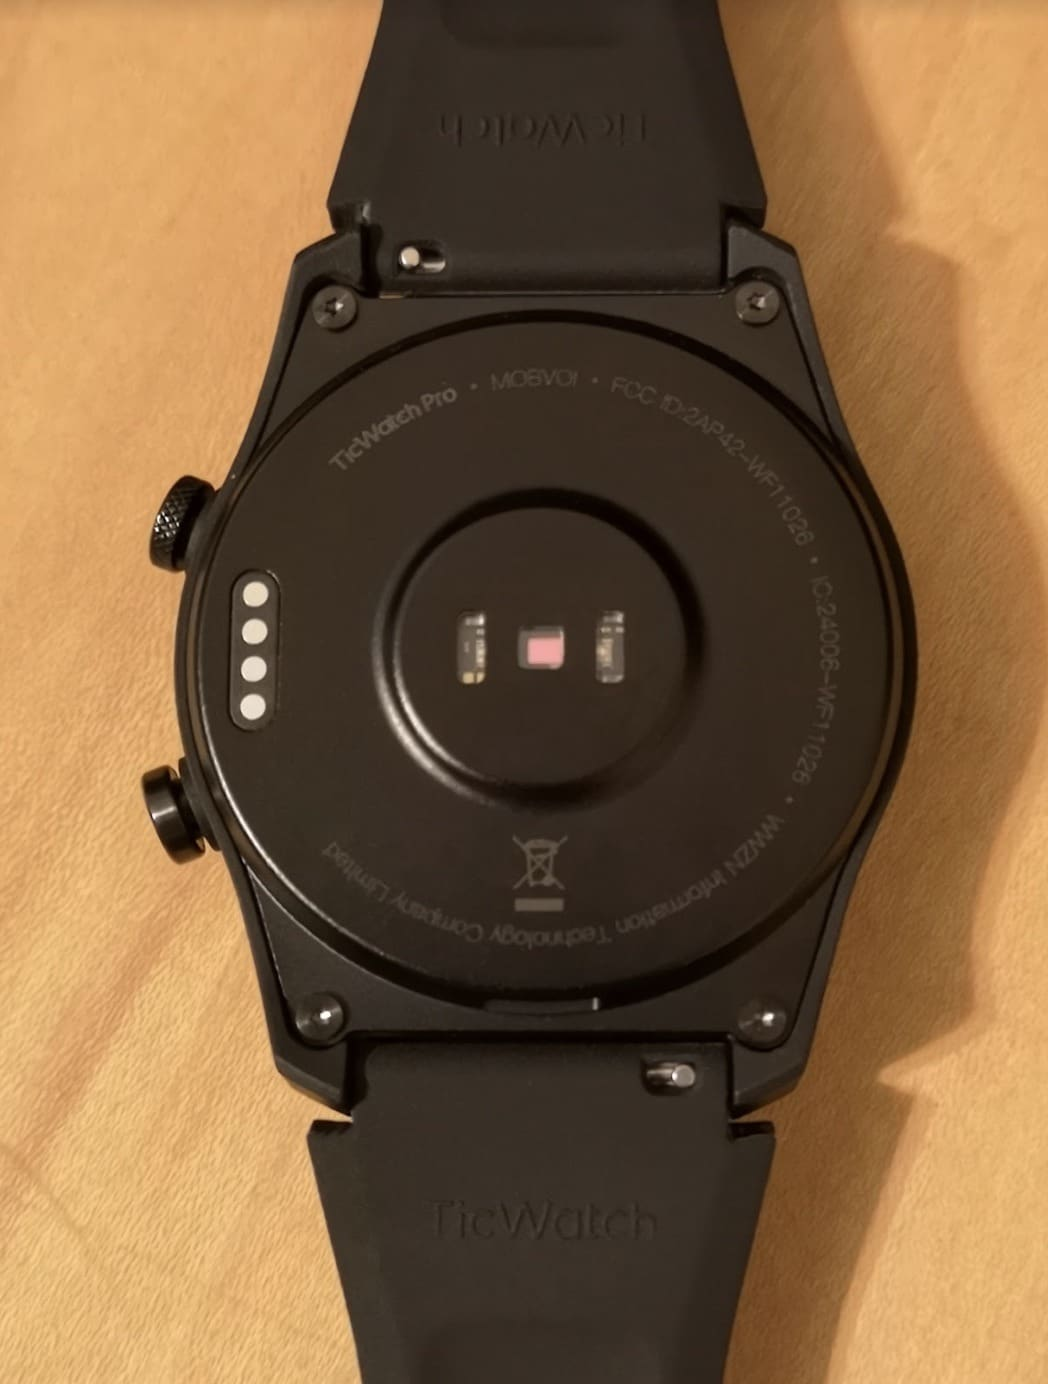
\includegraphics[width=0.26\textwidth]{chap4/image4/tikwatch1.jpg}}
  \caption[Ticwatch Smartwatch S2, Wear OS ]{Ticwatch Smartwatch S2, Wear OS\index{Hasnain}}
  \label{fig:Ticwatch}
\end{figure}
One of the main challenges is the design of a wearable, low-power, reliable and precise \acs{IoT} system. Commercial solutions also satisfy the criteria set out above.  One such solution is the fully wearable Ticwatch Smartwatch S2, Wear OS (shown in Fig.\ref{fig:Ticwatch}). The device has a Bluetooth module which allows communication with a suitable mobile application. This comes with no Google Fit API, as most commercial solutions do, and is thus programmable and customise able. Therefore, for real-time monitoring, further analytic, biofeedback, or integration with other educational services, there is possible to collect sensor data and store it in the Firebase database.

To maintain homeostasis, physical or mental imbalance induced by harmful stimuli can induce stress. The sympathetic nervous system is hyper activated during chronic stress which causes physical, psychological, and behavioral abnormalities. There is currently no accepted standard for assessing stress. This analysis aimed to survey studies that provide a basis for choosing variation in the \acf{HR} as a measure of psychological stress.\citep{Kim2018StressLiterature}

Your heart rate is changing from one minute to another. It depends on whether you stand or lie, move around or sit still, stressed or relaxed. Nonetheless, the restful heart rate continues to be steady every day. The usual heart rate resting range is between 60 and 90 beats per minute, anywhere. Over 90 is generally considered high.\citep{LeWine2011IncreasePublishing}
\subsection{\acf{SpO2}}
\acs{SpO2} stands for saturation of the peripheral capillary oxygen. It estimates how saturated the oxygen in your blood is. A safe, fit person usually sees a \acs{SpO2} ranging from 95\% to 100\%. Illness, altitude, heart disease, inhalation of smoke all have \acs{SpO2} effect.\citep{Sly2019ManagingBiostrap}
\begin{figure}[hbt!] 
  \centering
  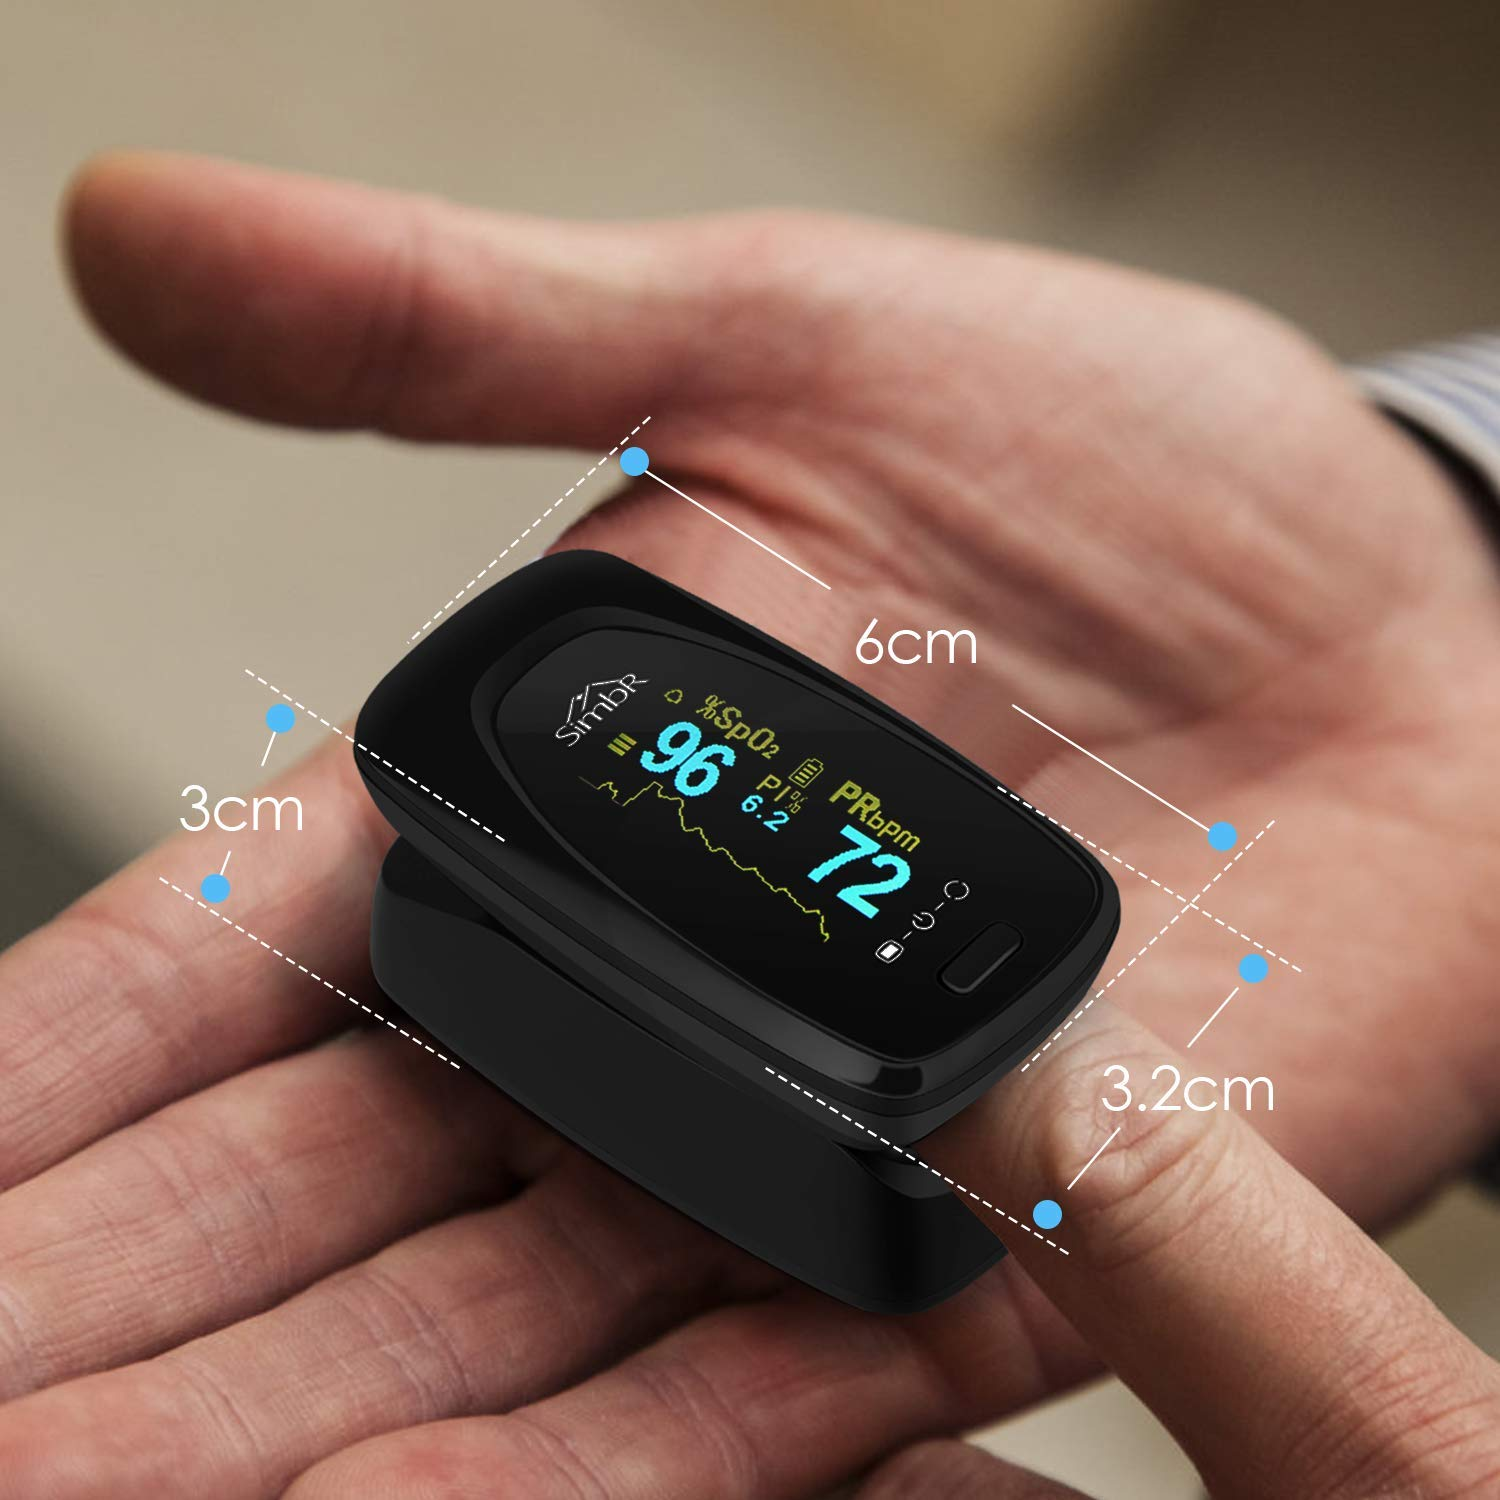
\includegraphics[width=0.6\linewidth]{chap4/image4/spo2.jpg}
  \caption[\acf{SpO2}]{\acf{SpO2}\index{Hasnain}}
  \label{fig:spo2}
\end{figure}
Your measure of \acs{SpO2} may not vary as much as your resting heart rate and HRV, but a sudden drop is often an indication of stress. Traditionally, athletes who train at higher altitudes track \acs{SpO2} to help make sure they get enough oxygen. This is an easy metric to track with the correct device along with the resting pulse.

\acs{SpO2} instant measurement device shows in figure:\ref{fig:spo2}. In this thesis we use this device for verifying the stress with personal feelings. And send data to cloud for further analysis and visualization.

\section{Symbolic Representation for Others}
Symbolic representation is basically a communicative activity that distinguishes human beings from other species and brings them together within cultures and other social groups. This section explores symbolic representation in our study, and we restrict our development to symbolic representation in the context of external symbols used in contact with others.
\begin{figure}[hbt!] 
  \centering
  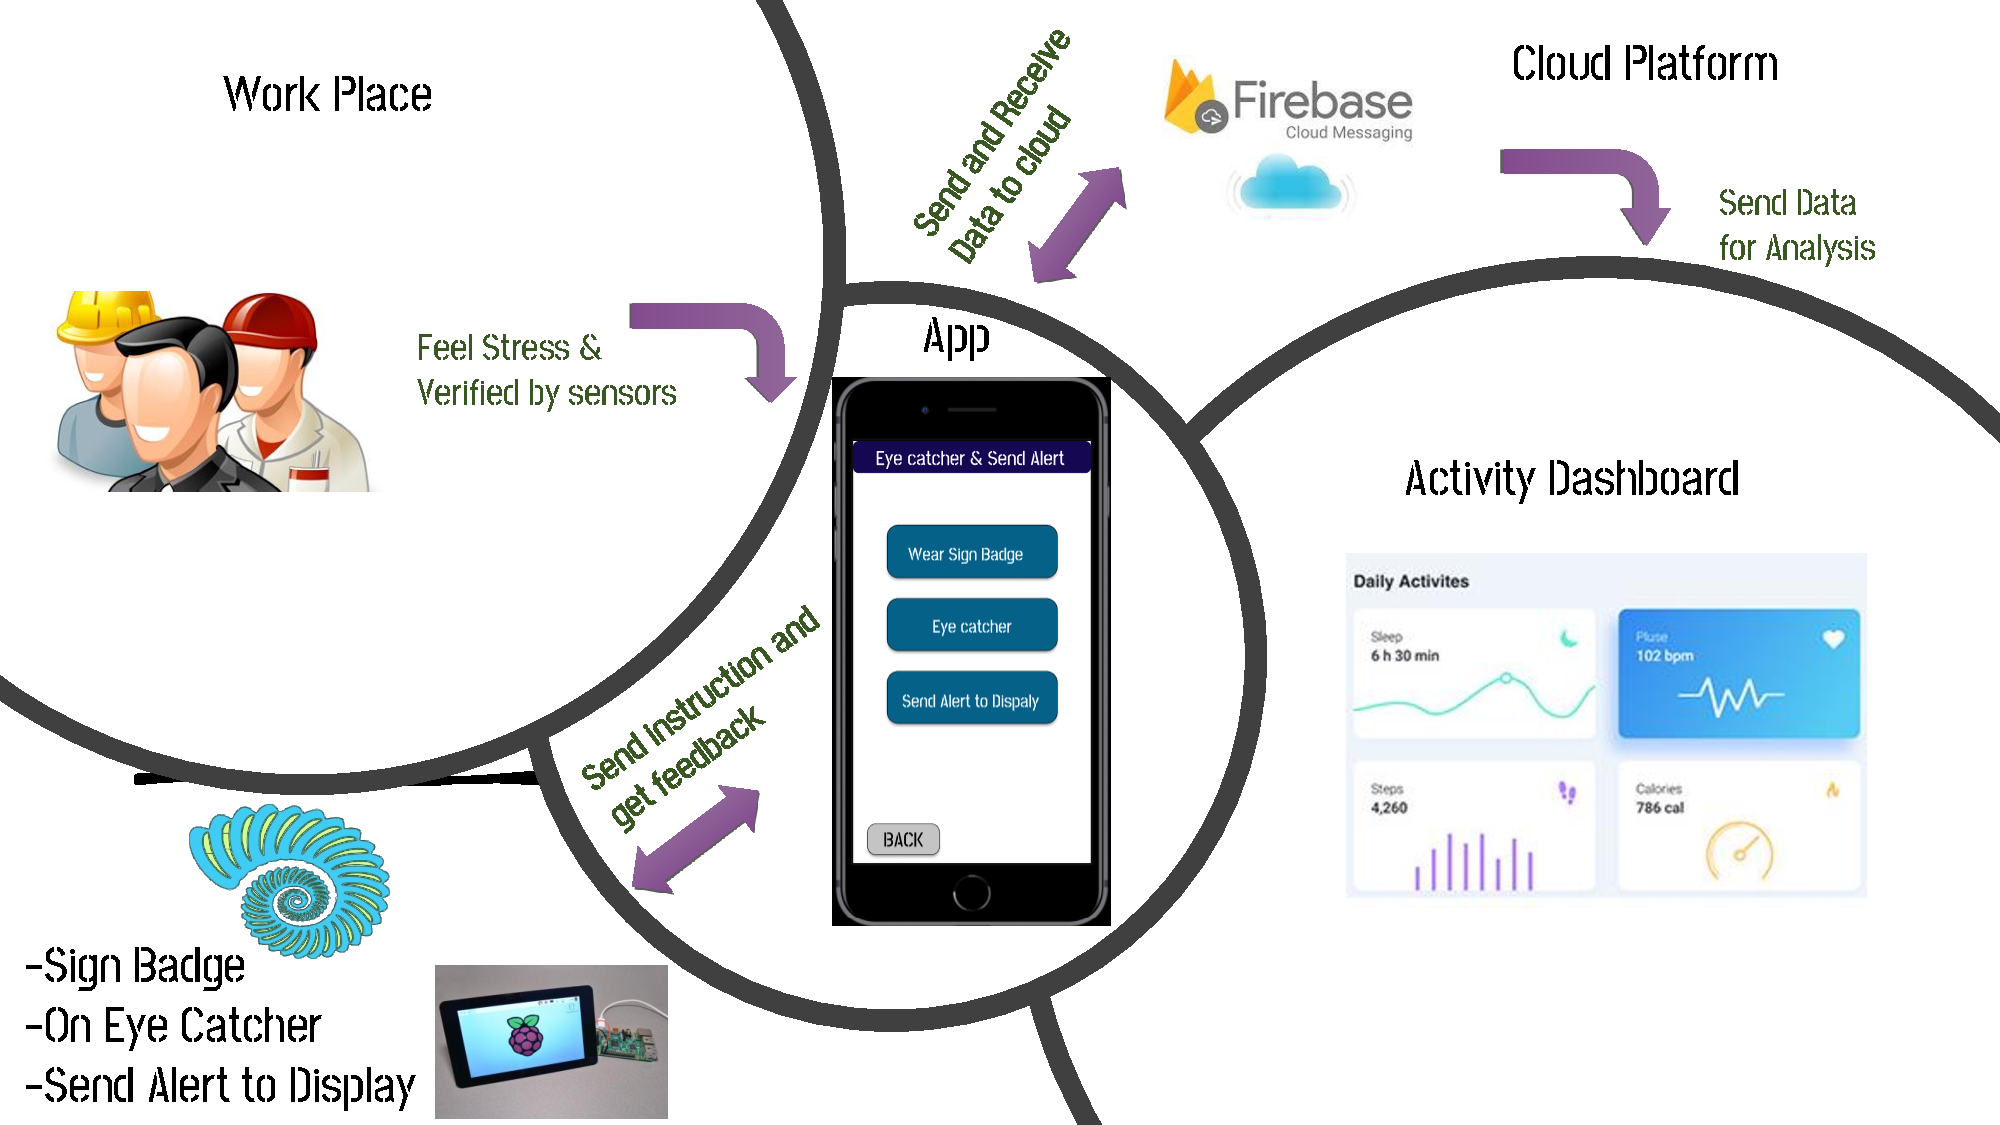
\includegraphics[width=1.0\linewidth]{chap4/image4/sign.pdf}
  \caption[Symbolic Representation for Others Process Diagram ]{Symbolic Representation for Others Process Diagram\index{Hasnain}}
  \label{fig:Sign}
\end{figure}
we used Three types of Symbolic representation for alert surrounding at work place.
\begin{itemize}
    \item Special Sign Badge
    \item Eye catcher
    \item Send Alerts to Wireless display
\end{itemize}

\subsection{Special Sign Badge}
In our thesis we use \textbf{Schneckenhaus} symbol badge as a metaphor of stressed condition.
\begin{figure}[hbt!] 
  \centering
  
\includegraphics[width=0.5\linewidth]{chap4/image4/logo1.png}
  \caption[Schneckenhaus symbol sign badge ]{Schneckenhaus symbol sign badge\index{Hasnain}}
  \label{fig:Sign_badge}
\end{figure}
\subsection{Eye catcher}
\begin{figure}[hbt!] 
  \centering
  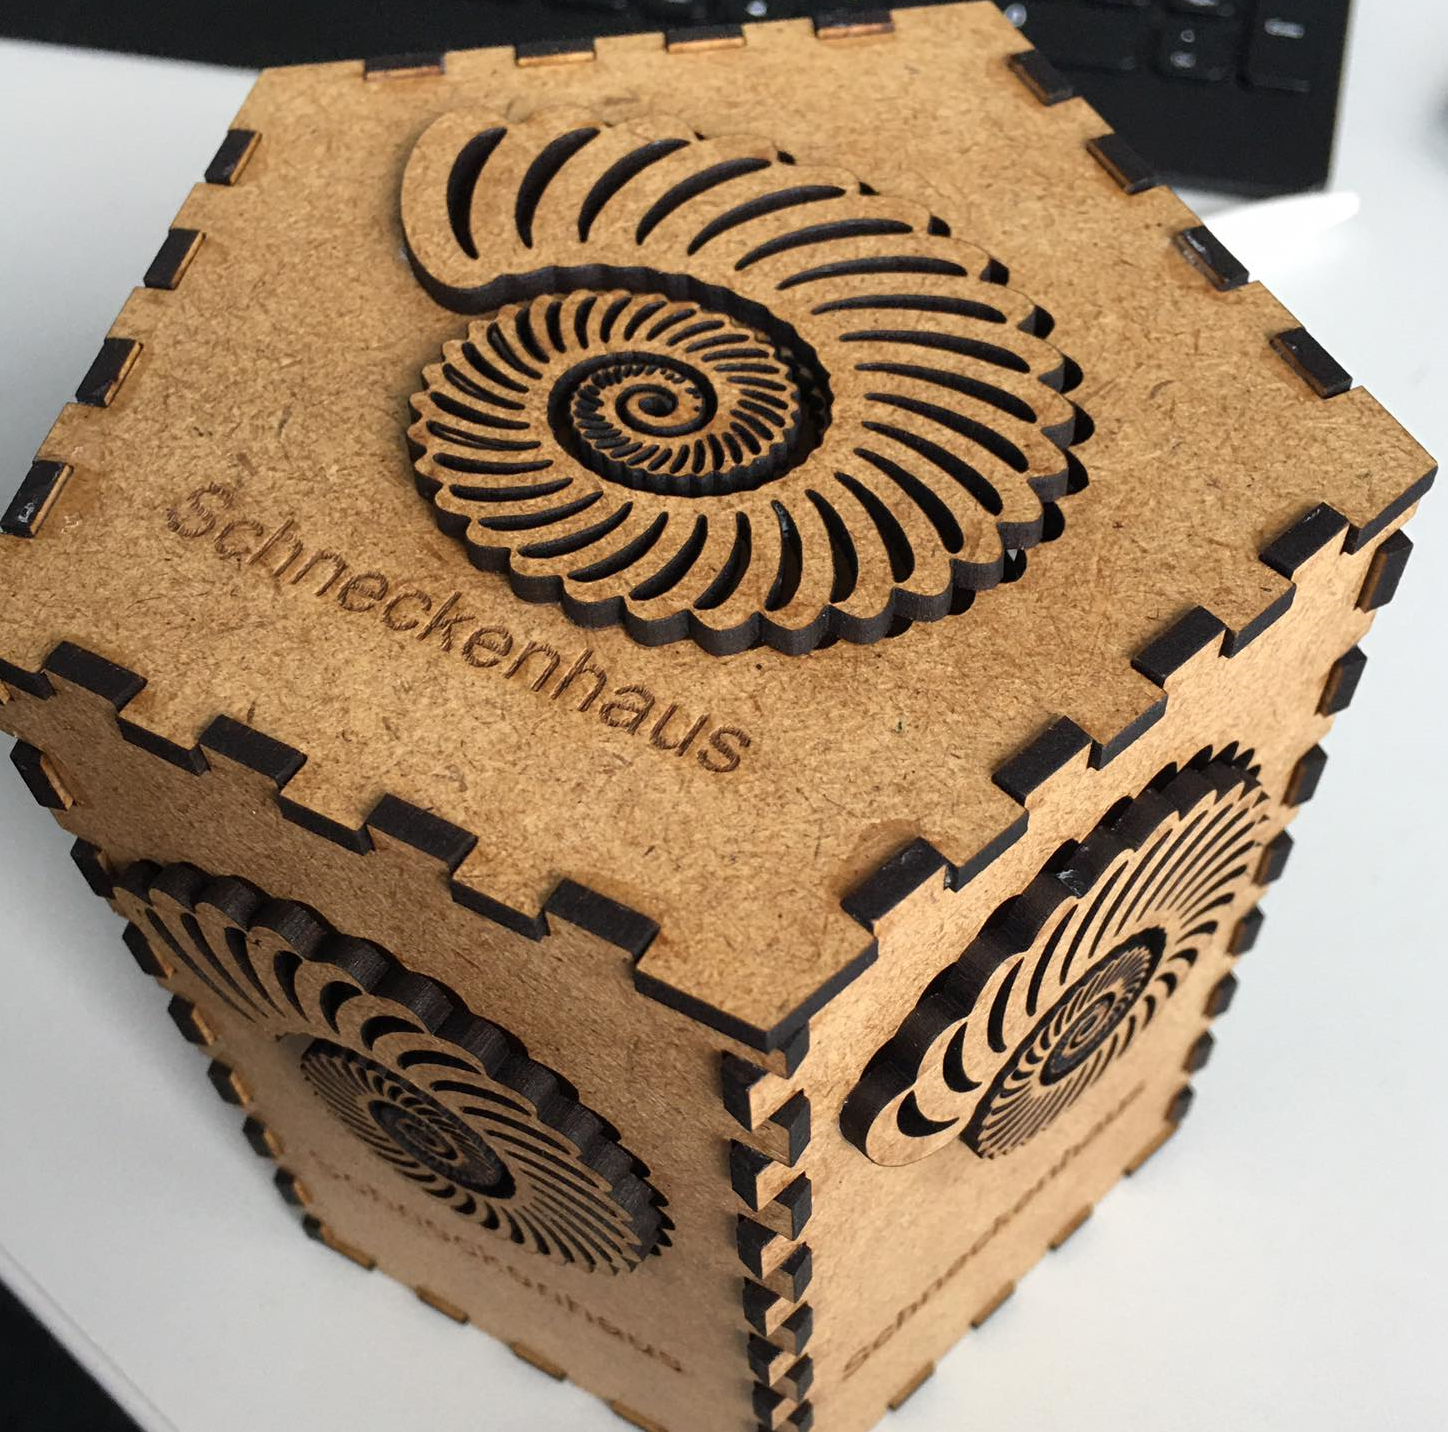
\includegraphics[width=0.5\linewidth]{chap4/image4/skn2.png}
  \caption[Eye catcher ]{Eye catcher\index{Hasnain}}
  \label{fig:eye}
\end{figure}
\subsection{Send Alerts to Wireless display}
\begin{figure}[hbt!] 
  \centering
  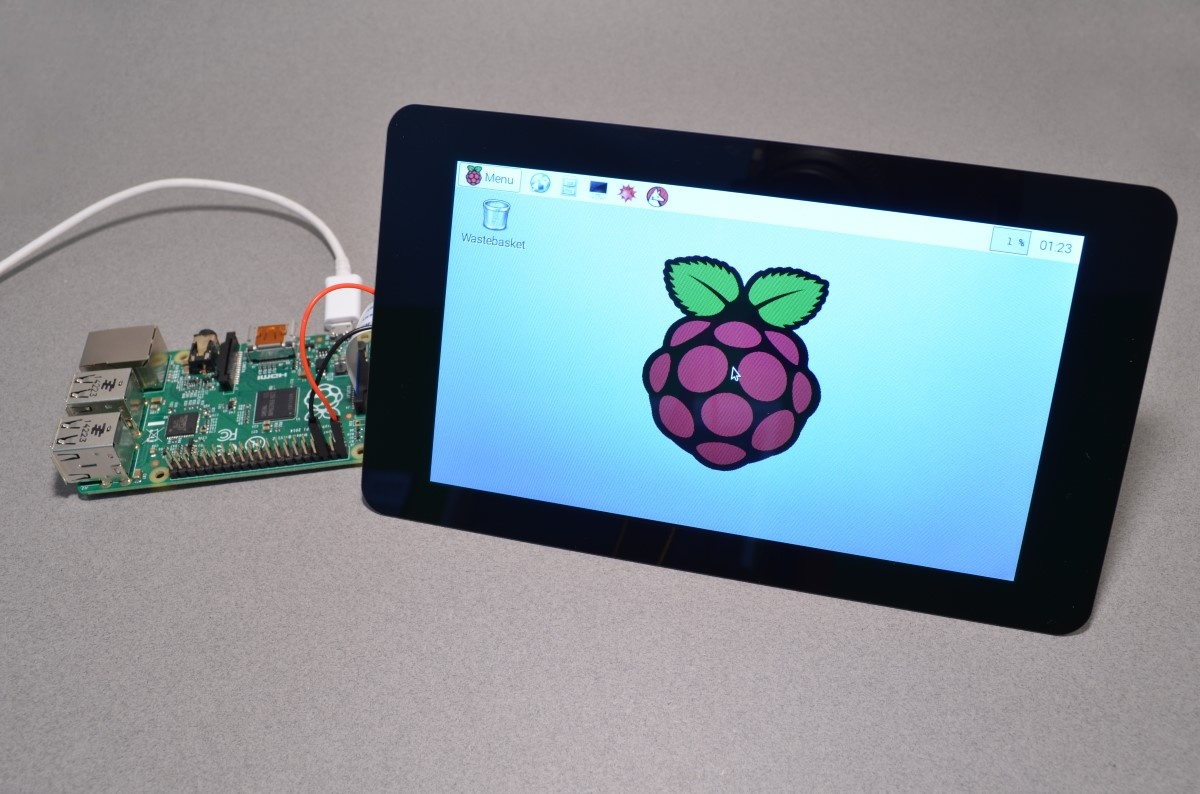
\includegraphics[width=0.5\linewidth]{chap4/image4/dipl.jpg}
  \caption[Raspberry PI Wireless display ]{Raspberry PI Wireless display\index{Hasnain}}
  \label{fig:PI_disp}
\end{figure}

\section{Interactive Chatbot}
A chatbot is an Artificial Intelligence (AI) program that simulates interactive human conversation using key pre-calculated user phrases and auditory or text based signals. Chatbots are often used for basic customer service and marketing systems which frequent hubs of social networking and instant messaging (IM) customers. They too are often included in operating systems as intelligent virtual assistants.

Also known as chatbot is an artificial conversational entity (ACE), chat robot, talk bot, chatter bot, or chatterbox.
\subsection{}
\section{Dashboard for data Visualization }
As in the database, we store only the meta information about the object hypothesis, so it is not understandable, which annotations are wrong. The framework also provides a javascript based visualization tool [12], which helps users to visualize the object hypothesis and the annotated information with it. There-
fore, user can understand, when the robot did mistake (recognize false positive,bad detection, segmentation errors etc.) during the perception task. So he can
take right measures for the errors. The web visualization tool is shown by the following figure.
\section{Empowerment}
